\documentclass[10pt,a4paper,twocolumn]{article}
\usepackage[T1]{fontenc}
\usepackage[utf8]{inputenc}
\usepackage{minted}
\usepackage{amsmath}
\usepackage{amsfonts}
\usepackage{amssymb}
\usepackage{fancyhdr}
\usepackage{graphicx, wrapfig, subcaption, setspace, booktabs}
\usepackage[font=small, labelfont=bf]{caption}
\usepackage[list=true]{subcaption}
\usepackage{url, lipsum}
\usepackage{hyperref}
\usepackage{listings}
\usepackage[dvipsnames]{xcolor}
\setlength\headheight{60pt}

\renewcommand{\figurename}{Figura}
\graphicspath{{figures/}}
\renewcommand{\headrulewidth}{2pt}
\definecolor{iselcolor}{rgb}{0.941,0.275 , 0.157} 
\definecolor{isel_beringela}{rgb}{0.37,0.08, 0.22} 
\renewcommand{\headrule}{\hbox to\headwidth{%
  \color{iselcolor}\leaders\hrule height \headrulewidth\hfill}}

\usepackage{lscape}

\renewcommand{\lstlistingname}{Algoritmo} % adjusts Listings caption and reference lst
\renewcommand{\lstlistlistingname}{Lista de Algoritmos}
\lstdefinelanguage{Kotlin}{
  comment=[l]{//},
  commentstyle={\color{gray}\ttfamily},
  emph={filter, first, firstOrNull, forEach, lazy, map, mapNotNull, println},
  emphstyle={\color{OrangeRed}},
  identifierstyle=\color{black},
  keywords={!in, !is, abstract, actual, annotation, as, as?, break, by, catch, class, companion, const, constructor, continue, crossinline, data, delegate, do, dynamic, else, enum, expect, external, false, field, file, final, finally, for, fun, get, if, import, in, infix, init, inline, inner, interface, internal, is, lateinit, noinline, null, object, open, operator, out, override, package, param, private, property, protected, public, receiveris, reified, return, return@, sealed, set, setparam, super, suspend, tailrec, this, throw, true, try, typealias, typeof, val, var, vararg, when, where, while},
  keywordstyle={\color{NavyBlue}\bfseries},
  morecomment=[s]{/*}{*/},
  morestring=[b]",
  morestring=[s]{"""*}{*"""},
  ndkeywords={@Deprecated, @JvmField, @JvmName, @JvmOverloads, @JvmStatic, @JvmSynthetic, Array, Byte, Double, Float, Int, Integer, Iterable, Long, Runnable, Short, String, Any, Unit, Nothing},
  ndkeywordstyle={\color{BurntOrange}\bfseries},
  sensitive=true,
  stringstyle={\color{ForestGreen}\ttfamily},
}

\begin{document}
\pagestyle{fancy}
\fancyhead{} % clear all header fields
\fancyhead[LO]{
\includegraphics[width=4cm]{01_ISEL-Logotipo-RGB_Horizontal-Compacto-900.png}}
\fancyhead[RO]{
\textbf{Port Expander LCD} (\textit{Ticket Machine}) \\ 
\footnotesize
Laboratório de Informática e Computadores 2025 / 2026 verão \\
Autores: Hugo Gomes / José Gaspar / Rafael Hipólito}
\fancyfoot{} % clear all footer fields
\fancyfoot[RO]{\thepage}


O módulo \textit{Port Expander LCD} (\textit{PELCD}) tem como principal objetivo realizar a interface entre o módulo de 
\textit{Control}, implementado em software, e o periférico LCD. 

O módulo \textit{PELCD} é constituído por um bloco único designado por \textit{Serial Receiver}, como representado na Figura 
\ref{fig:PortExpander}. 

Neste caso, o módulo \textit{Control} é a entidade produtora da informação, enquanto o \textit{LCD} atua como entidade consumidora.

\begin{figure}[H]
\begin{center}
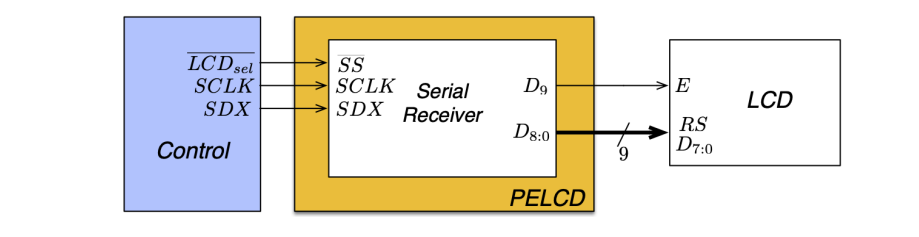
\includegraphics[width=0.48\textwidth]{figures/PortExpanderLCDDiagrama.png} 
\caption{Diagrama de blocos do módulo \textit{Port Expander LCD}}
\label{fig:PortExpander}
\end{center}
\end{figure} 

\section{Serial Receiver}

\noindent \par O bloco \textit{Serial Receiver} é responsável pela receção da informação enviada em série pelo módulo de 
\textit{Control}, armazenando os bits recebidos e disponibilizando-os posteriormente ao LCD sob a forma de sinais apresentados em série.

\noindent \par De acordo com o diagrama apresentado na Figura~\ref{fig:SerialReceiver}, este bloco integra dois sub-blocos principais:

\begin{itemize}
    \item um registo de deslocamento (\textit{Shift Register});
    \item um registo de manutenção (\textit{Hold Register}).
\end{itemize}

\begin{figure}[H]
\begin{center}
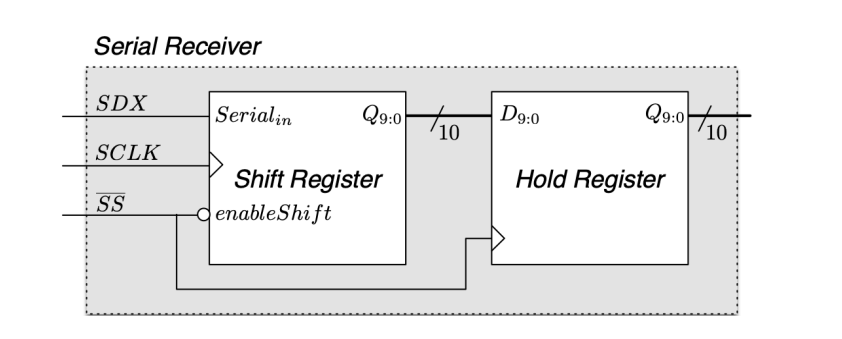
\includegraphics[width=0.48\textwidth]{figures/SerialReceiverDiagrama.png} 
\caption{Diagrama de blocos do módulo \textit{Serial Receiver}}
\label{fig:SerialReceiver}
\end{center}
\end{figure} 

\noindent \par A receção da informação é iniciada por uma transição descendente do sinal \textit{LCDsel}, conforme ilustrado na Figura~\ref{fig:ProtocolPELCD}, sendo os bits da trama recebidos sequencialmente até se totalizar a informação completa, que, posteriormente, é disponibilizada ao \textit{Hold Register}.

\noindent \par O sinal de \textit{enable} (\textit{E}), incluído na trama recebida, é utilizado para controlar o registo da informação no LCD. Este é gerado pelo módulo de \textit{Control}, sendo alternado entre duas tramas consecutivas.

\noindent \par A informação recebida pelo \textit{Serial Receiver} é organizada sob a forma de uma trama de 10 bits, constituída por um bit de seleção de registo (\textit{RS}), oito bits de dados e um bit de ativação (\textit{E}), sendo os bits transmitidos sequencialmente a partir do bit menos significativo. Esta organização permite, não só distinguir entre comandos (\textit{CMD}) e dados (\textit{DATA}), como também o modo como é controlado o registo da informação no LCD.

\begin{figure}[H]
\begin{center}
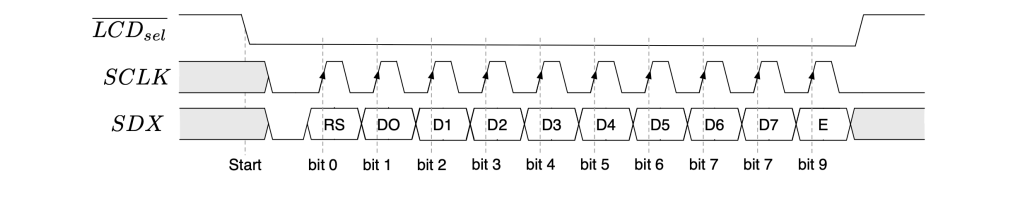
\includegraphics[width=0.48\textwidth]{figures/ProtocolComPELCD.png} 
\caption{Protocolo de comunicação com o módulo \textit{Port Expander LCD} (\textit{PELCD})}
\label{fig:ProtocolPELCD}
\end{center}
\end{figure} 

\subsection{Shift Register}

\noindent \par O \textit{Shift Register} é responsável pela receção sequencial dos bits de dados provenientes da entrada (\textit{SDX}). A cada transição ascendente do sinal (\textit{SCLK}), um novo bit é introduzido no registo, sendo o conteúdo previamente armazenado deslocado um bit para a direita. Este comportamento resulta da implementação deste registo como um conjunto de \textit{flip-flops} ligados em série.

\noindent \par Deste modo, o registo vai acumulando os bits recebidos até perfazer os 10 bits da trama enviada pelo módulo \textit{Control}, correspondendo à trama completa a disponibilizar ao \textit{Hold Register}.

\subsection{Hold Register}

\noindent \par O \textit{Hold Register} é responsável pelo armazenamento da palavra completa após a receção dos 10 bits da trama, provenientes do \textit{Shift Register}. Este registo mantém os valores estáveis e guardados, permitindo a sua correta aplicação ao \textit{LCD}.

\noindent \par Este bloco, à semelhança do \textit{Shift Register}, é implementado como um registo de 10 bits constituído por \textit{flip-flops}, que permitem armazenar simultaneamente todos os bits da informação recebida. Apesar desta semelhança, ao contrário do \textit{Shift Register}, neste registo os bits não são deslocados sequencialmente, todos os valores permanecem constantes até à receção de nova informação.

\noindent \par Os bits armazenados neste registo são diretamente aplicados às entradas do LCD, correspondendo ao sinal de seleção de registo (\textit{RS}), aos oito bits de dados e ao sinal de \textit{enable} (\textit{E}), responsável pelo registo da informação no \textit{LCD}.
\noindent \par Desta forma, garante-se também que os sinais aplicados ao \textit{LCD} permanecem estáveis durante o processo de escrita.




\section{Conclusões}

\noindent \par O módulo \textit{Port Expander LCD} permite realizar a interface entre o módulo de \textit{Control} e o \textit{LCD}, assegurando a correta receção e adaptação da informação enviada em série.
\noindent \par A utilização de uma arquitetura baseada num \textit{Serial Receiver}, constituído por um \textit{Shift Register} e um \textit{Hold Register}, permite separar o processo de receção sequencial do armazenamento estável da informação, garantindo a correta aplicação dos dados ao \textit{LCD}.
\noindent \par Através da comunicação série utilizada, é permitida a redução do número de linhas de interligação necessárias, simplificando o sistema sem comprometer a fiabilidade da transmissão. Desta forma, é garantida uma integração eficiente do módulo \textit{Port Expander LCD} na arquitetura global do sistema.

\onecolumn
\newpage
\section*{Referências}
\addcontentsline{toc}{section}{\protect\numberline{}Referências}
\begin{thebibliography}{9}
\bibitem{Slides das aulas}
Laboratório de Informática e Computadores - Slides de apoio às aulas, 2025/2026.

\bibitem{Enunciado}
Laboratório de Informática e Computadores - Enunciado do Projeto "Ticket Machine", 2025/2026.

\bibitem{guiaQuartus}
Pedro Miguens Matutino, Sérgio André \emph{Guia de Instalação do Quartus Prime Lite Edition 20.1.1.720}, 2022, ISEL.
\end{thebibliography}

\clearpage
\appendix
\section{VHDL}

\subsection{PELCD}
\label{sec:PELCD_VHDL}
\begin{minipage}{\linewidth}
\footnotesize
\inputminted{vhdl}{vhdl/PELCD.vhd}
\label{vhdl:PELCD}
\end{minipage}

\subsection{PELCD testbench}
\label{sec:PELCD_tb_VHDL}
\begin{minipage}{\linewidth}
\footnotesize
\inputminted{vhdl}{vhdl/PELCD_tb.vhd}
\label{vhdl:PELCD_tb}
\end{minipage}

\subsection{RG10}
\label{sec:RG10_VHDL}
\begin{minipage}{\linewidth}
\footnotesize
\inputminted{vhdl}{vhdl/RG10.vhd}
\label{vhdl:RG10}
\end{minipage}

\subsection{Serial Receiver}
\label{sec:SerialReceiver_VHDL}
\begin{minipage}{\linewidth}
\footnotesize
\inputminted{vhdl}{vhdl/SerialReceiver.vhd}
\label{vhdl:SerialReceiver}
\end{minipage}

\subsection{Serial Receiver testbench}
\label{sec:SerialReceiver_tb_VHDL}
\begin{minipage}{\linewidth}
\footnotesize
\inputminted{vhdl}{vhdl/SerialReceiver_tb.vhd}
\label{vhdl:SerialReceiver_tb}
\end{minipage}

\subsection{Shift Register}
\label{sec:shiftRegister_VHDL}
\begin{minipage}{\linewidth}
\footnotesize
\inputminted{vhdl}{vhdl/ShiftReg.vhd}
\label{vhdl:shiftRegister}
\end{minipage}

\subsection{Shift Register testbench}
\label{sec:shiftRegister_tb_VHDL}
\begin{minipage}{\linewidth}
\footnotesize
\inputminted{vhdl}{vhdl/ShiftReg_tb.vhd}
\label{vhdl:shiftRegister_tb}
\end{minipage}

\clearpage
\section{\textit{Kotlin}}
\subsection{LCD}
\lstinputlisting[language=Kotlin, basicstyle=\scriptsize, caption={LCD - Liquid Cristal Display}, label={lst:LCD}]{kotlin/LCD.kt}

\subsection{SerialEmitter}
\lstinputlisting[language=Kotlin, basicstyle=\scriptsize, caption={Serial Emitter}, label={lst:SerialEmitter}]{kotlin/SerialEmitter.kt}


\end{document}